% -----------------------------------------------------------------------------
% Implementation
% -----------------------------------------------------------------------------
\chapter{Implementation}

As noted before the ANC system has solely been implemented in the simulation environment Matlab. The system consist of several subsystems. These subsystems will be elaborated step by step and their functioning will be demonstrated.\\
The complete source code can be found in the \color{blue}\href{https://github.com/leonardberresheim/MA---Active-Noise-Control-in-Spatial-Domains/tree/main/Matlab}{projects github repository} \color{black} and is free to use, change and share without restrictions.



\section{Spherical Harmonics Decomposition}
The accuracy of the spherical harmonics decomposition in (\ref{eq:primary_noise_field}) with it's truncation degree will be demonstrated using a plane wave \textit{(see figure \ref{fig:planeWaveExp}}) as the exact harmonic coefficients can be calculated using (\ref{eq:plane_wave_coefficients}).
\begin{figure}
    \centerline{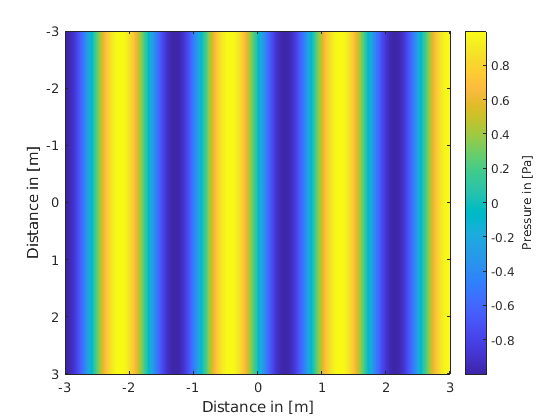
\includegraphics{LaTeX/images/plots/plane_Wave_exponent_form.png}}
    \caption{Plane wave in exponent form}
    \label{fig:planeWaveExp}
\end{figure}

\begin{figure}
    \centerline{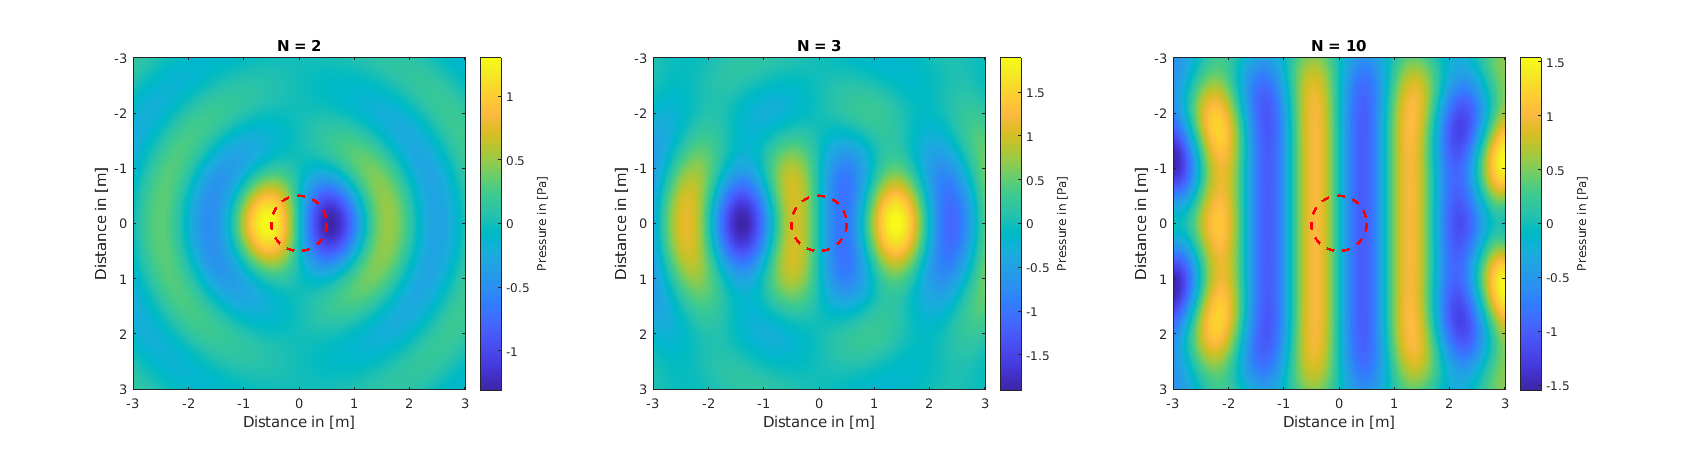
\includegraphics[width=\paperwidth]{LaTeX/images/plots/Plane_wave_harmonics_form.png}}
    \caption{Plane wave in harmonics form for number of modes 2, 3 and 10}
    \label{fig:planeWaveHarmonics}
\end{figure}
When increasing the number of modes the resulting noise field gets closer and closer to the original plane wave in figure \ref{fig:planeWaveExp} as can be seen in figure \ref{fig:planeWaveHarmonics}. However only the quiet zone (\textit{marked as a red circle}) is of interest and with a higher number of modes the number of required loudspeakers increase as well as the computation time. In fact figure \ref{fig:planeWaveHarmonicsError} shows that in the region of interest the accuracy of the spherical harmonics decomposition for $N = 3$ is already adequate.
\begin{figure}
    \centerline{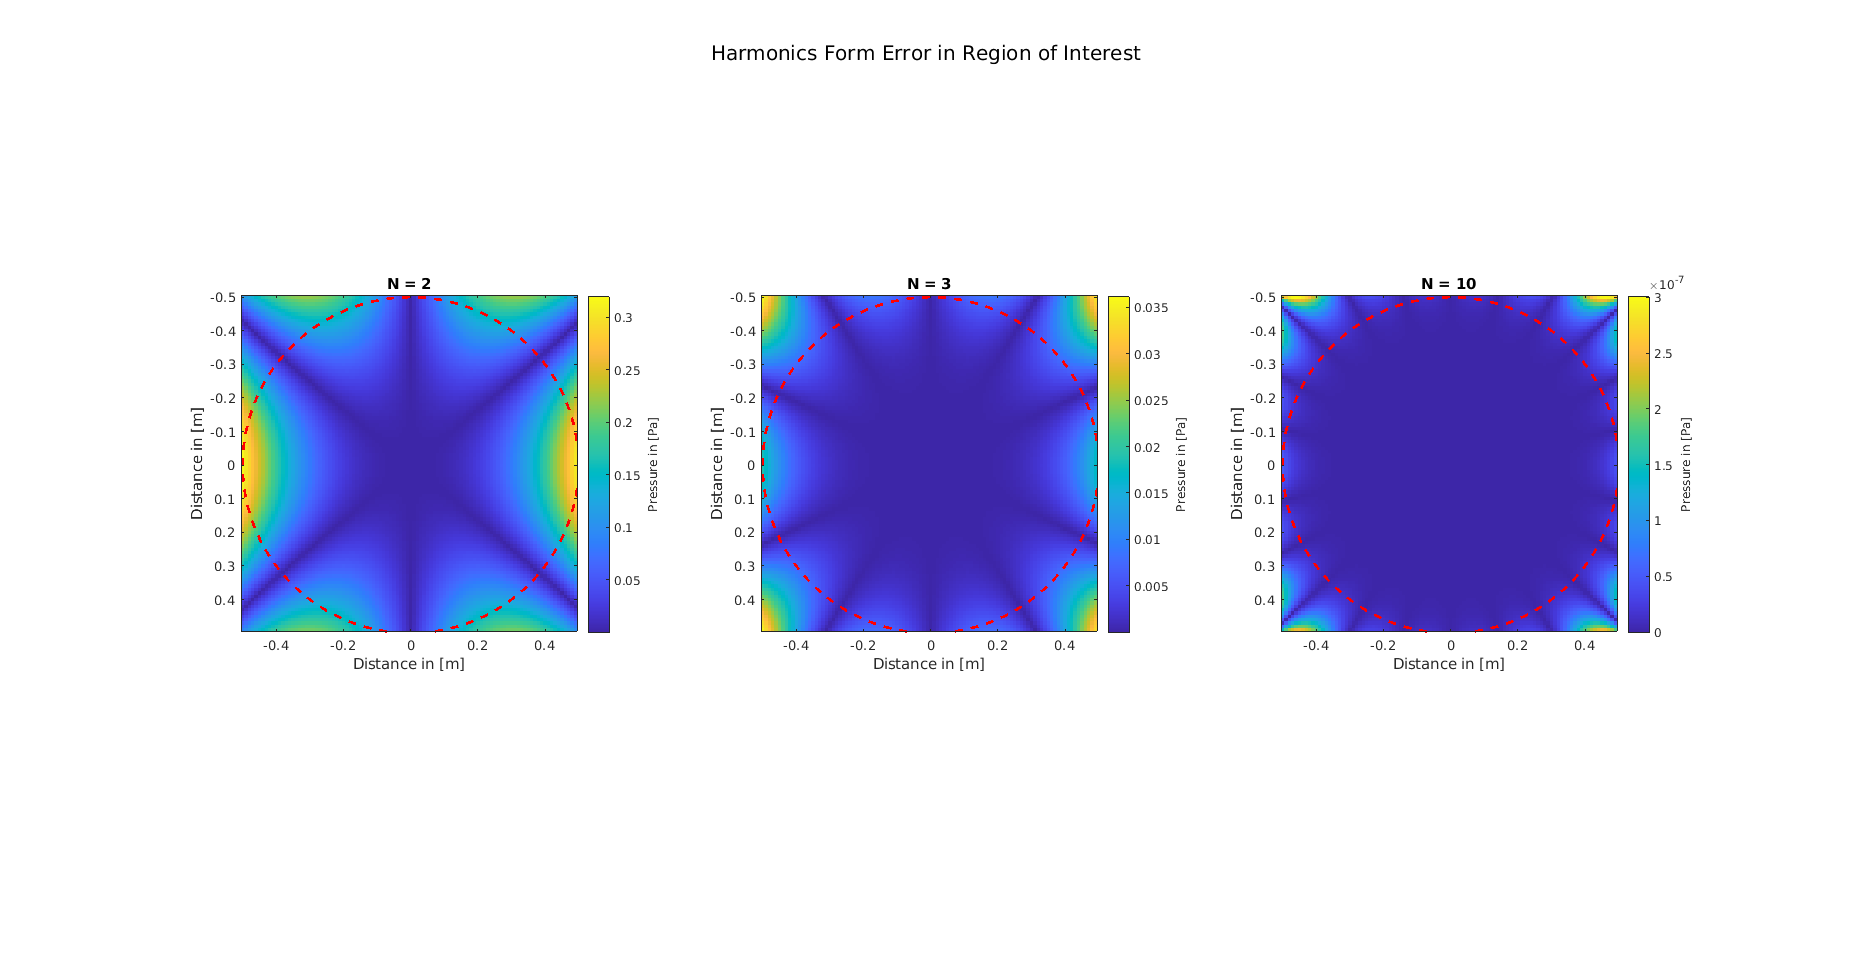
\includegraphics[width=\paperwidth]{LaTeX/images/plots/Plane_wave_harmonics_form_Error.png}}
    \caption{Error of the plane wave in harmonics form within region of interest for number of modes 2, 3 and 10}
    \label{fig:planeWaveHarmonicsError}
\end{figure}
\\
\\
\textit{Nota}\\
Only the imaginary part is plotted here as the behavior of the real part of the wave is analogous.
\section{Spherical Microphone Array}
The spherical microphone array is setup around the region of interest according to the Gaussian sampling scheme discussed in \textit{section \ref{sec:Gaussian}} with $2(N+1) = 8$ microphones on the azimuth angle in line with (\ref{eq:azimuth_sample}) and $(N + 1) = 4$ microphones on the elevation angle in line with (\ref{eq:elevation_sample}) resulting in a total of $2(N + 1)^2 = 32$ microphones arranged on the sphere \textit{(see figure \ref{fig:MicrophoneArray}})
\begin{figure}
    \centerline{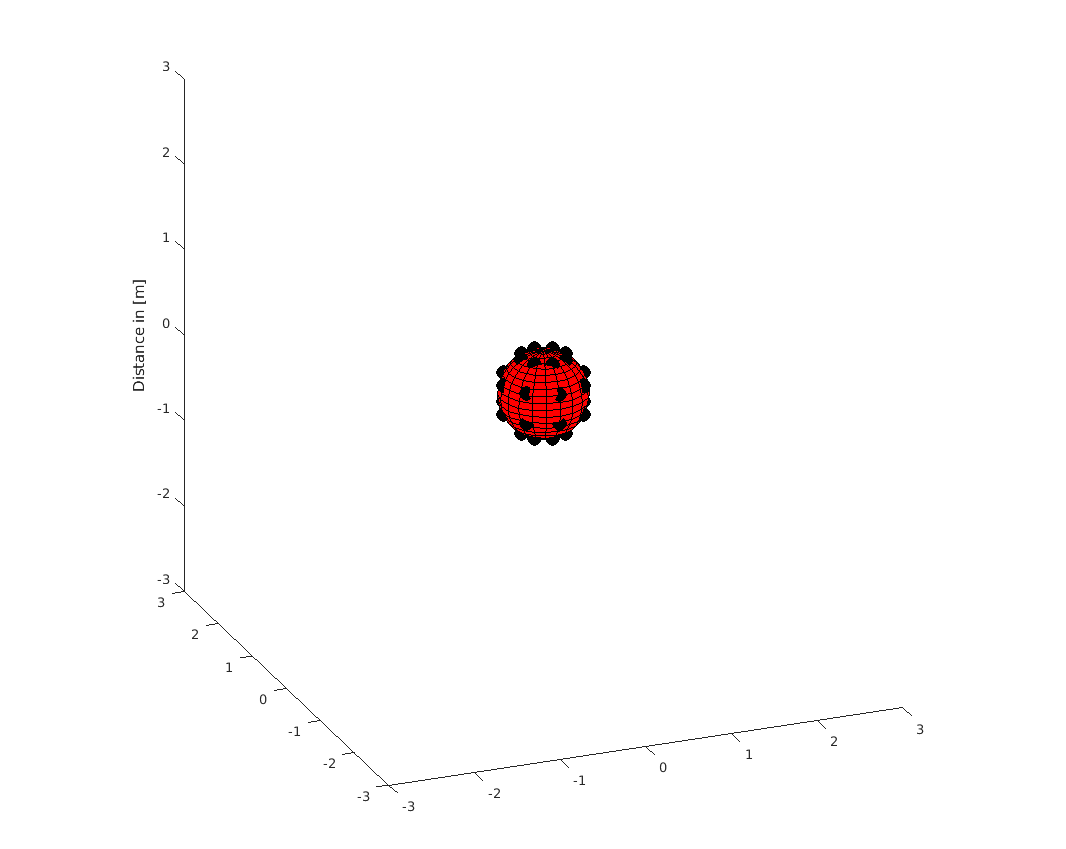
\includegraphics[width=\paperwidth]{LaTeX/images/plots/MicrophoneArray.png}}
    \caption{Spherical microphone array arranged according to the Gaussian sampling scheme}
    \label{fig:MicrophoneArray}
\end{figure}
\section{Approximation of Harmonic Coefficient}
Applying the Gaussian sampling scheme discussed in \textit{section \ref{sec:Gauss}}, the sampling weights are set according to (\ref{eq:gauss_weights}) and the harmonic coefficients for the noise field generated by the plane wave are approximated using (\ref{eq:gauss_harmonic_coefficients}).


\begin{figure}
    \centerline{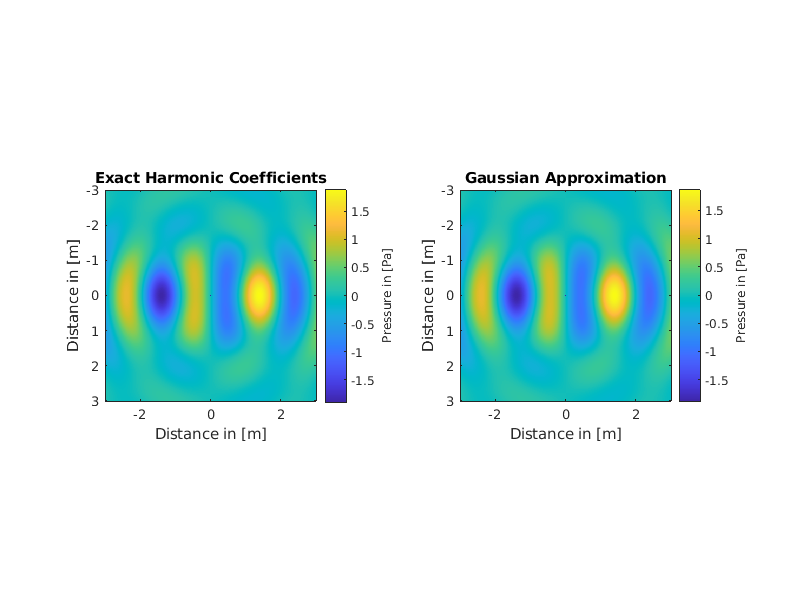
\includegraphics[width=\paperwidth]{LaTeX/images/plots/Gauss_Approcimation.png}}
    \caption{Plane wave noise field approximation in the wave domain with exact harmonic coefficients and Gaussian sampling approximation for N = 3}
    \label{fig:GaussianApproximation}
\end{figure}

The resulting noise field approximation using the Gaussian sampling scheme appears very similar to the exact noise field approximation\textit{(see figure \ref{fig:GaussianApproximation}}.\\
Surprisingly the error of the Gaussian approximation in regards to the actual plane wave is lesser at the corners than for the exact approximation as can be seen in figure \ref{fig:GaussianApproximationError}.\\\\

\textit{Nota}\\
By \textit{exact} the analytical solution to the harmonic coefficient from (\ref{eq:plane_wave_coefficients}) in consideration of the truncation order of $N = 3$ is meant. 


\begin{figure}
    \centerline{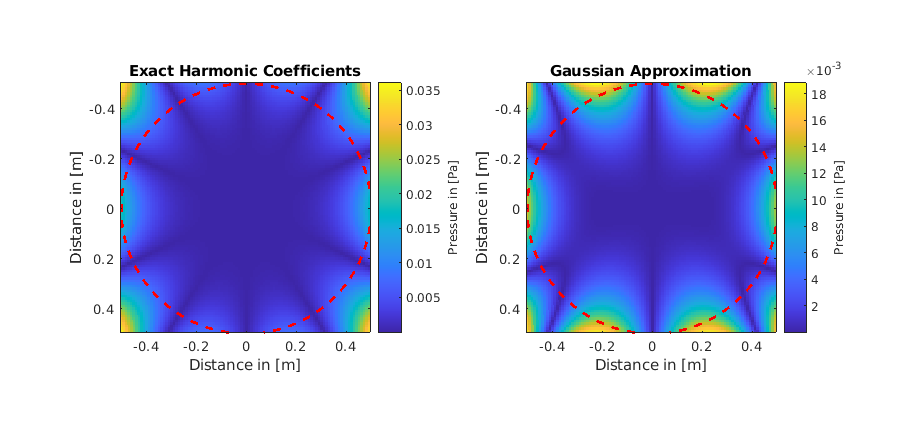
\includegraphics[width=\paperwidth]{LaTeX/images/plots/Gauss_Approximation_Error.png}}
    \caption{Error for the plane wave noise field approximation in the wave domain with exact harmonic coefficients and Gaussian sampling approximation for N = 3}
    \label{fig:GaussianApproximationError}
\end{figure}

\section{Simulation Setup}
The simulation setup is set in accordance with \cite{Zhang2019}. The environment is modeled by a \textit{shoebox} room of $6m \times 6m \times 6m$ with reflection coefficients at [0.75,0.8,0.77,0.85,0.1,0.1] which are usual for a common room with relatively high reflection coefficients for the walls and relatively low reflection coefficients for floor and ceiling. The source is modeled as a point source as defined by (\ref{eq:point_source}. For now we assume the noise field to contain only a single frequency component and the point source to emit at a constant magnitude of 10.\\ The region of interest is spherical area of radius $R_1 = 0.5m$ located at the origin which as seen in \textit{section \ref{sec:primary}} leads to a number of modes of $N = \lceil ekR_1/2\rceil = 3$. As depicted in \textit{section \ref{sec:matching}} $(N+1)^2 = 16$ loudspeaker would be necessary to bear an exact solution. But as aforementioned and discussed \textit{Case 3} will be realized in which the number of loudspeaker is lesser and thus an approximation is required. The number of loudspeaker is set to 12 as seen in figure \ref{fig:setup}.

\begin{figure}
    \centerline{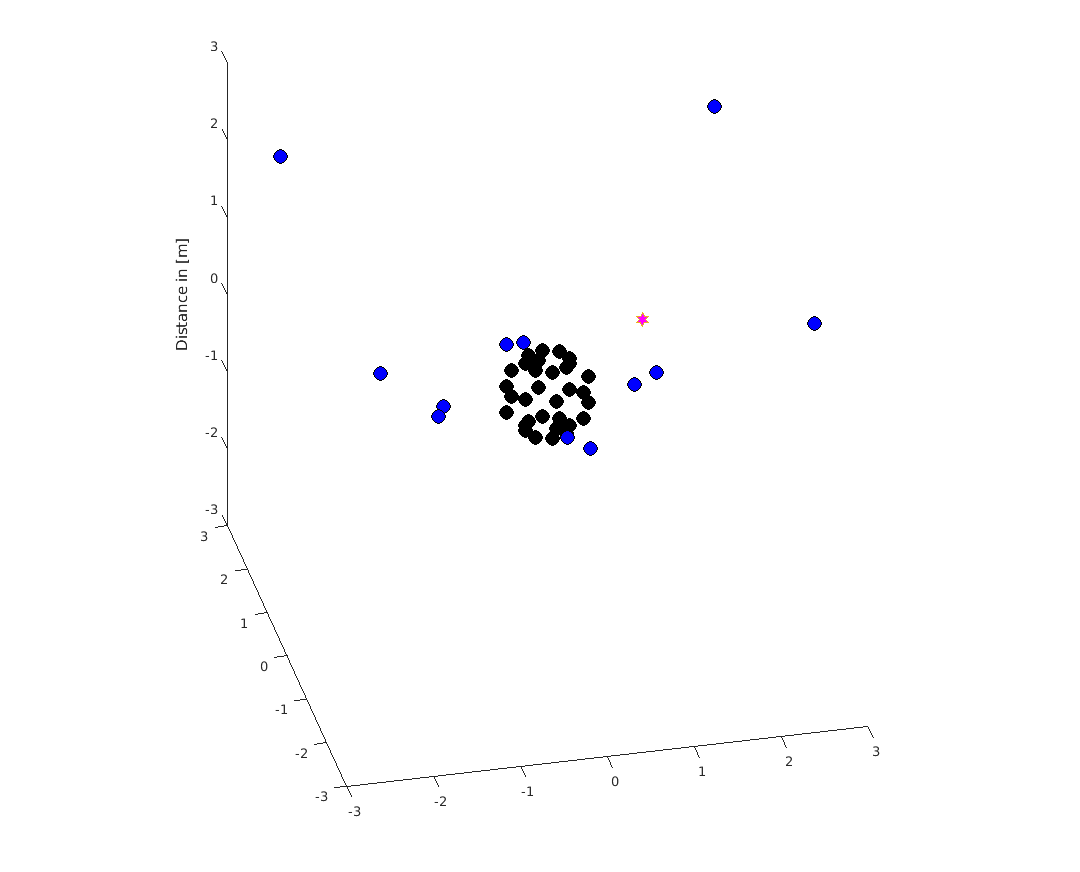
\includegraphics[width=\paperwidth]{LaTeX/images/plots/ANCSetup.png}}
    \caption{Simulation setup, where the blue points are the loudspeaker positions, the pink star is the noise source position and the black points represent the microphones positions}
    \label{fig:setup}
\end{figure}

\section{Point Source Reverberation}


\begin{figure}
    \centerline{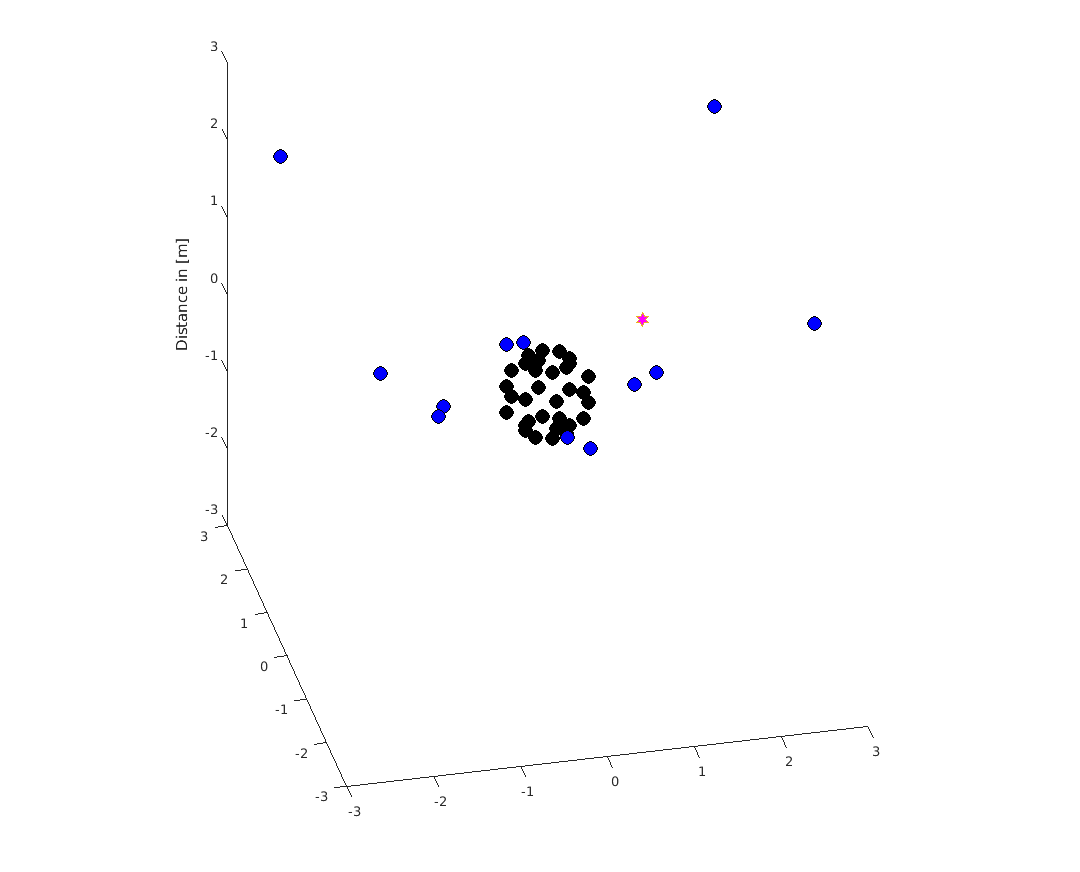
\includegraphics[width=\paperwidth]{LaTeX/images/plots/ANCSetup.png}}
    \caption{Simulation setup, where the blue points are the loudspeaker positions, the pink star is the noise source position and the black points represent the microphones positions}
    \label{fig:setup}
\end{figure}